\chapter{Сегментація зображення для прискорення алгоритмів стереобачення}

У третьому розділі запропоновано метод прискорення алгоритмів стереобачення,
що використовує сегментацію зображення.

\section{Сегментація зображення}

Ліве зображення $L$ зі вхідної стереопари
розбивається на прямокутну решітку з однаковим заданим розміром комірок.
Усі пікселі, що належать одній комірці,
діляться на дві групи за середньою інтенсивністю пікселів комірки
(рис.~\ref{fig:superpixels:visualization}).
До першої групи (зображена білим на рисунку) відносять пікселі,
інтенсивність яких не перевищує середньої інтенсивності пікселів комірки.
Піксель із координатами $\left(x^*, y^* \right)$, що належить даній комірці $S$
потрапляє до першої групи, якщо
\begin{equation*}
    L \left(x^*, y^* \right) \le
        \frac{1}{ \left| S \right| }
        \sum \limits_{\left(x, y \right) \in S} L \left(x, y \right),
\end{equation*}
де $ \left| S \right|$~---~кількість пікселів у комірці.
До другої групи, що зображена чорним на рисунку,
відносять усі інші пікселі комірки, що не потрапили в першу групу.
Кожну таку групу будемо називати \textit{суперпікселем}.
Отже, у процесі сегментації ліве зображення
стереопари розбивається на комірки, у яких міститься два суперпікселя:
більш світлий і більш темний.

\begin{figure}[h]
\centering
    \begin{subfigure}[t]{0.3\textwidth}
        \centering
        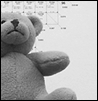
\includegraphics[width=\textwidth]{images/cell}
        \caption{Комірка зображення}
        \label{fig:cell}
    \end{subfigure}
    \qquad
    \begin{subfigure}[t]{0.3\textwidth}
        \centering
        
\includegraphics[width=\textwidth]{images/superpixels}
        \caption{Комірка зображення, розбита на два суперпікселя}
        \label{fig:superpixels}
    \end{subfigure}
    \caption{Візуалізація суперпікселів}
    \label{fig:superpixels:visualization}
\end{figure}

Після запропонованої сегментації будується
$\left| T_s \right|$-дольний граф з множиною координат суперпікселів
\begin{equation*}
    T_s = \left\{
        \left(x_s, y_s, i \right) \; \middle| \;
        1 \le x_s \le m, \,
        1 \le y_s \le n, \,
        i \in \left\{ 0, 1 \right\}
    \right\},
\end{equation*}
де $m$~---~кількість комірок по горизонталі,
$n$~---~кількість комірок по вертикалі,
$i$~---~індекс суперпікселя.
Тепер кожній долі графу відповідає один суперпіксель~---~об'єкт графу.
Кожен об'єкт $\left(x_s, y_s, i \right) \in T_s$ містить
$ \left| D \right|$ міток (або вершин),
які відповідають усім можливим зсувам горизонтальної координати пікселів,
що належать об'єкту.
Отже, всі пікселі, що належать одному суперпікселю,
будуть мати однакову глибину (або зсув) на результуючій карті глибин,
тобто тепер горизонтальний зсув $d \in D$
буде шукатися не для кожного пікселя окремо, а для цілої групи пікселів,
які утворюють суперпіксель, одночасно.

В об'єкті $\left(x_s, y_s, i \right) \in T_s$ на вершину з міткою $d \in D$
накладається штраф,
який дорівнює сумі штрафів за вибір відповідних вершин у всіх пікселях,
які належать даному суперпікселю,
\begin{equation*}
    f_{\left(x_s, y_s, i\right)}^s \left( d \right) =
    \sum \limits_{\left(x, y \right) \in \left(x_s, y_s, i \right)}
        f_{\left(x, y \right)} \left( d \right),
\end{equation*}
де $f_{\left(x, y \right)} \left( d \right)$~---~штраф за вибір вершини,
введений у першому розділі дисертації у формулі \eqref{eq:penalty:vertex}.

Кожен об'єкт може мати до дев'яти сусідів: по два об'єкти у верхній, правій,
нижній і лівій комірках, а також другий об'єкт,
який належить тій же комірці (рис.~\ref{fig:superpixel:neighbors}).
Об'єкти, що відповідають коміркам на краях зображення, мають по сім сусідів,
а об'єкти, що відповідають кутовим коміркам,~---~по п'ять.
Штраф, який накладається на дужки між вершинами різних об'єктів, такий же,
як і при постановці задачі без суперпікселів, тобто дорівнює
$g_{\left(x_s, y_s, i \right), \left(x_s', y_s', i' \right)}
    \left(d, d' \right)$,
де $\left(x_s, y_s, i \right) \in T_s$ та
$\left(x_s', y_s', i' \right) \in T_s$~---~сусідні об'єкти,
$d$~---~мітка в об'єкті $\left(x_s, y_s, i \right)$,
а $d'$~---~мітка в об'єкті $\left(x_s', y_s', i' \right)$.
Множину всіх пар сусідніх об'єктів в цьому графі позначимо через $\mathcal{N}^s$.

\begin{figure}[h]
  \centering
  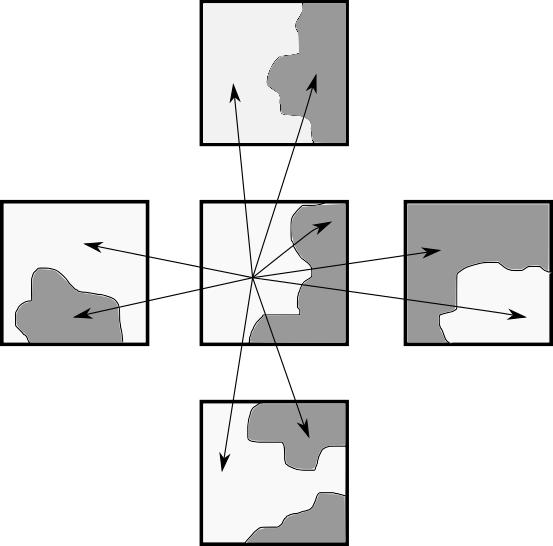
\includegraphics[width=0.7\textwidth]{images/neighbours_superpixel}
  \caption{Структура сусідства при використанні суперпікселів.
           Квадратами позначені комірки,
           що містять по два суперпікселя (об'єкта):
           світлий ($i = 0$) і темний ($i = 1$).
           Стрілками позначені дуги,
           що виходять зі світлого суперпікселя центральної комірки в об'єкти,
           що є для нього сусідніми}
  \label{fig:superpixel:neighbors}
\end{figure}

Аналогічно штрафній функції \eqref{eq:overview:penalty}
вихідної задачі отримуємо штрафну функцію модифікованої задачі
\begin{equation*}
\begin{gathered}
    G_s \left( \pmb{d} \right)
    = \sum \limits_{x = 1}^{m}
        \sum \limits_{y = 1}^{n}
            \sum \limits_{i \in \left\{ 0, 1 \right\}}
                f_{\left( x_s, y_s, i \right)}^s
                    \left( d \left(x_s, y_s, i \right) \right) + \\
    + \sum \limits_{\left( \left(x_s, y_s, i \right), \left(x_s', y_s', i' \right) \right) \in \mathcal{N}^s}
            g_{\left(x_s, y_s, i \right), \left(x_s', y_s', i' \right)} \left(
                d \left( x_s, y_s, i \right), d \left( x_s', y_s', i' \right)
            \right).
\end{gathered}
\end{equation*}

Далі задача розв'язується методом, що описаний у попередньому розділі,
тобто максимізується дуальна функція Лагранжа \eqref{eq:lagrange:dual:MAP}
за допомогою алгоритму дифузії,
а потім застосовується алгоритм викреслювання
другого порядку для знаходження оптимальної розмітки.

\section{Оцінка складності алгоритму дифузії}

Без використання сегментації зображення складність
одного елементарного кроку алгоритму дифузії,
що складається з двох операцій \eqref{eq:diffusion:first} та
\eqref{eq:diffusion:second} для одного об'єкта $\left(x, y \right) \in T$
дорівнює $\mathcal{O} \left( \left| D \right|^2 \right)$.

Складність однієї ітерації алгоритму дифузії,
що полягає у виконанні елементарного кроку для всіх об'єктів,
дорівнює $\mathcal{O} \left(\left|T \right| \cdot \left|D\right|^2 \right)$.

Після сегментації алгоритм дифузії залишається без змін,
відрізняється лише розмір графу та кількість дуальних змінних,
за якими йде максимізація.
Складність однієї ітерації алгоритму дифузії
після сегментації зображення дорівнює
$\mathcal{O} \left( \left| T_s \right| \cdot \left| D^2 \right| \right)$.
Кількість об'єктів $\left| T_s \right|$ дорівнює кількості прямокутних комірок,
на які було розбито зображення, помноженої на $2$,
бо кожна комірка містить два об'єкта (суперпікселя).
Тому $\left| T_s \right| = 2 \cdot m \cdot n$,
де $m$~---~кількість комірок по горизонталі,
$n$~---~кількість комірок по вертикалі.
Оскільки всі комірки мають однакові розміри, то
\begin{equation*}
    \left| T_s \right| =
    2 \cdot m \cdot n =
    2 \cdot \frac{w}{w_c} \cdot \frac{h}{h_c} =
    2 \cdot \frac{\left| T \right|}{w_c \cdot h_c},
\end{equation*}
де $w_c$~---~ширина комірки, $h_c$~---~висота комірки.
Отже, складність однієї ітерації алгоритму дифузії після
сегментації зображення складає
\begin{equation} \label{eq:diffusion:superpixel:complexity}
    \mathcal{O} \left(
        \frac{\left| T \right|}{w_c \cdot h_c} \cdot \left| D \right|^2
    \right).
\end{equation}

При сегментації зображення складність однієї ітерації алгоритму дифузії
зменшується пропорційно площі комірок, на які розбивається зображення.
Чим більший розмір комірки, тим менше об'єктів містить граф,
і складність алгоритму дифузії зменшується.
При цьому зменшується кількість змінних $\varphi$,
по яким максимізується дуальна функція Лагранжа \eqref{eq:lagrange:dual:MAP}.

\section*{Висновки до розділу 3}
\addcontentsline{toc}{section}{Висновки до розділу 3}

Запропоновано спосіб прискорення алгоритмів,
які використовуються для розв'язання задачі стереобачення.
Прискорення базується на зменшенні розміру графу,
на якому розв'язується задача, за допомогою сегментації зображення так,
щоби не сильно погіршити результуючу карту глибин.
Параметром методу є розмір комірок, на які розбивається зображення.
